\documentclass[a4paper]{article}

\usepackage[english]{babel}
\usepackage{hyperref}
\usepackage[fleqn]{amsmath}
\usepackage{array}
\usepackage{graphicx}

\title{\textbf{Growth and Regional Development}\\ Lewis Model Assignment}

\begin{document}
\date{14-3-2016}
\author{}
\maketitle
\begin{center}
\author{\bf Berend Stofferis}\\
ANR: 941240\\
\href{mailto: B.J.Stofferis@uvt.nl}{B.J.Stofferis@uvt.nl}\\
\end{center}
\thispagestyle{empty}

\newpage
\tableofcontents
\newpage
\section{Derivation of the Lewis Model}
Before we turn to the main questions of the assignment, we first build up the Lewis model. We will derive the most important equations for reference later on. Start by writing down the seven equations that form the blueprint of the Lewis design:
\begin{align}
	& Y_s=A_sL_s\\
	& w_s=A_s\\
    & Y_m=A_mK{^\alpha}L_m^{1-\alpha}\\
    & w_m=(1-\alpha)Y_m/L_m\\
    & L=L_m+L_s\\
    & w_m={\phi}w_s\\
    & \dot{K}=s_{\pi}[Y_m-w_mL_m]-{\delta}K
\end{align}
We presume the meaning of all variables are known by the reader. In short, there are tow sectors, a subsistence sector (subscript $s$) and a mature sector (subscript $m$). Only the mature sector works with capital, which is accumulated by saving a part of 'profits (perhaps profits is somewhat a misnomer, total income of capitalists is meant). Over time, labour moves from the subsistence sector to the mature sector as a response to the wage gap determined by ${\phi}$.

\subsection{Static Equilibria}

First consider the labour market. Start with equation (3) and rewrite as follows to find an expression for $L_m$ that only depends on $K$:
\begin{alignat}{2}
	&			  && \hspace{0.1cm} w_m=(1-{\alpha})Y_m/L_m \nonumber\\
	& \Rightarrow && \hspace{0.1cm} L_m=(1-{\alpha})Y_m/w_m \nonumber\\
    & \Rightarrow && \hspace{0.1cm} L_m=(1-{\alpha})A_mK^{\alpha}L_m^{1-{\alpha}}/w_m \nonumber\\
    & \Rightarrow && \hspace{0.1cm} L_m=(1-{\alpha})A_mK^{\alpha}L_m^{1-{\alpha}}/{\phi}w_s \nonumber\\
    & \Rightarrow && \hspace{0.1cm} L_m=(1-{\alpha})A_mK^{\alpha}L_m^{1-{\alpha}}/{\phi}A_s \nonumber\\
    & \Rightarrow && \hspace{0.1cm} L_m=K((1-{\alpha})A_m/{\phi}A_s)^{1/{\alpha}}
\end{alignat}
Then by equation (5):
\begin{alignat}{2}
	& 	&& \hspace{0.1cm} L_s=L_m \nonumber\\
	& \Rightarrow && \hspace{0.1cm} L_s=L-K((1-{\alpha})A_m/{\phi}A_s)^{1/{\alpha}}
\end{alignat}
Both (8) and (9) are only valied if $L_m<L$. This is equivalent to:
\begin{alignat}{2}
	& && \hspace{0.1cm} K((1-{\alpha})A_m/{\phi}A_s)^{1/{\alpha}}<L \nonumber\\
	& \Rightarrow && \hspace{0.1cm} K<L-K({\phi}A_s/(1-{\alpha})A_m)^{1/{\alpha}}\hspace{0.1cm}{\equiv}\hspace{0.1cm}K^{\#}
\end{alignat}
\newpage \noindent
Where $K^{\#}$ is the amount of capital at the point where the economy reaches maturity: no longer any labour is employed in the subsistence sector. Next, turn to output. Using the labour market equilibria, we can rewrite equation (1) and (3):
\begin{align}
 Y_s &= A_sL_s \nonumber\\
 &= A_sL-A_sK((1-{\alpha})A_m/{\phi}A_s)^{1/{\alpha}}\\
 & \nonumber\\
 Y_m &= A_mK{^\alpha}L_m^{1-\alpha} \nonumber\\
 &= A_mK^{\alpha}(K((1-{\alpha})A_m/{\phi}A_s)^{1/\alpha})^{1-\alpha}\nonumber\\
 &= KA_m((1-{\alpha})A_m/{\phi}A_s)^{(1-\alpha)/\alpha}
\end{align}
Since we work with a Cobb-Douglas production function in the mature sector, profits simply equal a fraction ${\alpha}$ of $Y_m$:
\begin{align}
 Y_m-w_mL_m &= A_sL_s \nonumber\\
 &={\alpha}KA_m((1-{\alpha})A_m/{\phi}A_s)^{(1-\alpha)/\alpha}
\end{align}
Finally, total output $Y$ is defined as the sum of oputput in both sectors:
\begin{align}
 Y &= Y_s+Y_m \nonumber\\
 &= A_sL-A_sK((1-{\alpha})A_m/{\phi}A_s)^{1/{\alpha}}\nonumber\\ 
 &\hspace{0.4cm}+KA_m((1-{\alpha})A_m/{\phi}A_s)^{(1-\alpha)/\alpha} \nonumber\\
 &= A_sL-A_sK((1-{\alpha})A_m/{\phi}A_s)^{1/{\alpha}}\nonumber\\
 &\hspace{0.4cm}+KA_s({\phi/(1-\alpha)})((1-{\alpha})A_m/{\phi}A_s)^{1/\alpha} \nonumber\\
 &= A_sL+KA_s({\phi/(1-\alpha)-1})((1-{\alpha})A_m/{\phi}A_s)^{1/\alpha}
\end{align}

\subsection{Dynamics}

Above we have found formulations for labour supply (per sector), output, profits and wages as a function of $K$ and a bundle of exogenous variables. Since equation (7) specifies how $K$ moves over time, we can analyse the dynamics of the mentioned factors. First substitute profits as given by (13) into the capital accumulation equation and rewrite in terms of growth rates.
\begin{subequations}
\begin{alignat}{2}
 &\dot{K} 	&&=s_{\pi}[Y_m-w_mL_m]-{\delta}K \nonumber\\
 &{}		&&={\alpha}s_{\pi}KA_m((1-{\alpha})A_m/{\phi}A_s)^{(1-\alpha)/\alpha}-{\delta}K\\ 
 \Rightarrow \hspace{0.1cm} 
 &\hat{K}	&&={\alpha}s_{\pi}A_m((1-{\alpha})A_m/{\phi}A_s)^{(1-\alpha)/\alpha}-{\delta}
\end{alignat}
\end{subequations}
Note how the growth rate of capital is completely determined by exogenous variables (i.e. it is just a constant). Labour supply in the mature sector grows at the same rate as capital (as long as $L_m<L$):
\begin{subequations}
\begin{alignat}{2}
 &\dot{L}_m &&=\dot{K}((1-{\alpha})A_m/{\phi}A_s)^{1/{\alpha}}\\
 \Rightarrow \hspace{0.1cm} 
 &\hat{L}_m	&&=(\dot{K}((1-{\alpha})A_m/{\phi}A_s)^{1/{\alpha}})/(K((1-{\alpha})A_m/{\phi}A_s)^{1/{\alpha}})\nonumber\\
 &{}		&&=\hat{K}
\end{alignat}
\end{subequations}
\newpage
\noindent Subsistence sector income should shrink over time, feeding the growing mature sector with labour:
\begin{subequations}
\begin{alignat}{2}
 &\dot{Y}_s &&=-\dot{K}A_s((1-{\alpha})A_m/{\phi}A_s)^{1/{\alpha}}\\
 \Rightarrow \hspace{0.1cm} 
 &\hat{Y}_s	&&=-\frac{\dot{K}A_s((1-{\alpha})A_m/{\phi}A_s)^{1/{\alpha}}}{A_sL-A_sK((1-{\alpha})A_m/{\phi}A_s)^{1/{\alpha}}}\nonumber\\
 &{}		&&=-\hat{K}\frac{A_s((1-{\alpha})A_m/{\phi}A_s)^{1/{\alpha}}}{A_sL/K-A_s((1-{\alpha})A_m/{\phi}A_s)^{1/{\alpha}}}
\end{alignat}
\end{subequations}
\begin{subequations}
\begin{alignat}{2}
 &\dot{Y}_m &&=\dot{K}A_m((1-{\alpha})A_m/{\phi}A_s)^{(1-\alpha)/{\alpha}}\\
 \Rightarrow \hspace{0.1cm} 
 &\hat{Y}_m	&&=\frac{\dot{K}A_m((1-{\alpha})A_m/{\phi}A_s)^{(1-\alpha)/{\alpha}}}{KA_m((1-{\alpha})A_m/{\phi}A_s)^{(1-\alpha)/{\alpha}}}\nonumber\\
 &{}		&&=\hat{K}
\end{alignat}
\end{subequations}
Because both inputs in the mature sector grow at rate $\hat{K}$, income in the mature sector does as well. Moreover, since profits are just a fraction of mature income, it shares the same growth rate $\hat{K}$. We conclude this section by deriving total income growth.
\begin{subequations}
\begin{alignat}{2}
 &\dot{Y} &&=\dot{K}A_s(\phi/(1-\alpha)-1)((1-{\alpha})A_m/{\phi}A_s)^{1/{\alpha}}\\
 \Rightarrow \hspace{0.1cm} 
 &\hat{Y}	&&=\dot{K}A_s(\phi/(1-\alpha)-1)((1-{\alpha})A_m/{\phi}A_s)^{1/{\alpha}}/Y\nonumber\\
 &{}		&&=\frac{\dot{K}A_s(\phi/(1-\alpha)-1)((1-{\alpha})A_m/{\phi}A_s)^{1/{\alpha}}}{A_sL+KA_s({\phi/(1-\alpha)-1})((1-{\alpha})A_m/{\phi}A_s)^{1/\alpha}}\nonumber\\
 &{}		&&=\hat{K}\frac{A_s(\phi/(1-\alpha)-1)((1-{\alpha})A_m/{\phi}A_s)^{1/{\alpha}}}{A_sL/K+A_s({\phi/(1-\alpha)-1})((1-{\alpha})A_m/{\phi}A_s)^{1/\alpha}}\nonumber\\
 &{}		&&=\hat{K}\frac{A_sL/K+A_s(\phi/(1-\alpha)-1)((1-{\alpha})A_m/{\phi}A_s)^{1/{\alpha}}}{A_sL/K+A_s({\phi/(1-\alpha)-1})((1-{\alpha})A_m/{\phi}A_s)^{1/\alpha}}\nonumber\\
 &{}		&&\hspace{0.4cm}-\hat{K}\frac{A_sL/K}{A_sL/K+A_s({\phi/(1-\alpha)-1})((1-{\alpha})A_m/{\phi}A_s)^{1/\alpha}}\nonumber\\
 &{}		&&=\hat{K}(1-\frac{A_sL}{A_sL+KA_s({\phi/(1-\alpha)-1})((1-{\alpha})A_m/{\phi}A_s)^{1/\alpha}})\nonumber\\
  &{}		&&=\hat{K}(1-A_sL/Y)
\end{alignat}
\end{subequations}
Note how the factor $A_sL/Y$ becomes smaller over time, leading to an increasing growth rate of total income.
\newpage
\section{Saving Rate Assumptions}
\textit{The Lewis model assumes that a fixed fraction of profits is reinvested; the Solow model assumes that a fixed fraction of total income is reinvested. Let’s compare the two assumptions: how does the Lewis model change if the Solow assumption about savings rates is used and vice versa? Show the dynamics of the models.}\\
\newline
When connecting the Solow model and the Lewis model, the main issue is the different approach both models take with respect to the saving rate. In order to illustrate this, we use the following notation:
\begin{itemize}
\item \hspace{0.1cm}$s$ \hspace{1cm}the saving rate as a fraction of total income (i.e. $Y_m+Y_s$). \vspace{-0.1cm}
\item \hspace{0.1cm}$s_{Y_m}$ \hspace{0.59cm}the saving rate as a fraction of mature sector income. \vspace{-0.1cm}
\item \hspace{0.1cm}$s_{\pi}$ \hspace{0.81cm}the saving rate as a fraction of profits.
\end{itemize}
Superscript $L$ and $S$ are used when referring to the Lewis model and the Solow model, respectively. If we reformulate the general assumptions of both paradigms in these terms, the Solow model usually specifies $s^S$, whereas the Lewis model normally works with $s_{\pi}^L$. Now suppose, perhaps naively, that we equalize these saving rates, such that $s^S=s_{\pi}^L$. To make these saving rates more easily comparable, we first rewrite  in terms of a saving rate as a percentage of total income $s^L$. Note that:
\begin{alignat}{2}
	&{}							&&s_{\pi}^L[Y_m-w_mL_m]={\alpha}s_{\pi}^LY_m={\alpha}s_{\pi}^L(Y_m/Y)Y=s^LY\nonumber\\
    &\Rightarrow\hspace{0.1cm}	&&s^L={\alpha}s_{\pi}^L(Y_m/Y)
\end{alignat}
At the maturity point of the economy, where $K=K^{\#}$, it holds that $Y_m=Y$ by definition. Therefore $s^L={\alpha}s_{\pi}^L$ at the transition point between Lewis and Solow. Yet for $K>K^{\#}$, note that $s^L>{\alpha}s_{\pi}^L$, which implies that the graph of the saving rate as a function of $K$ makes a sudden hike at $K^{\#}$. Visually:
\newline
\begin{figure}[!ht]
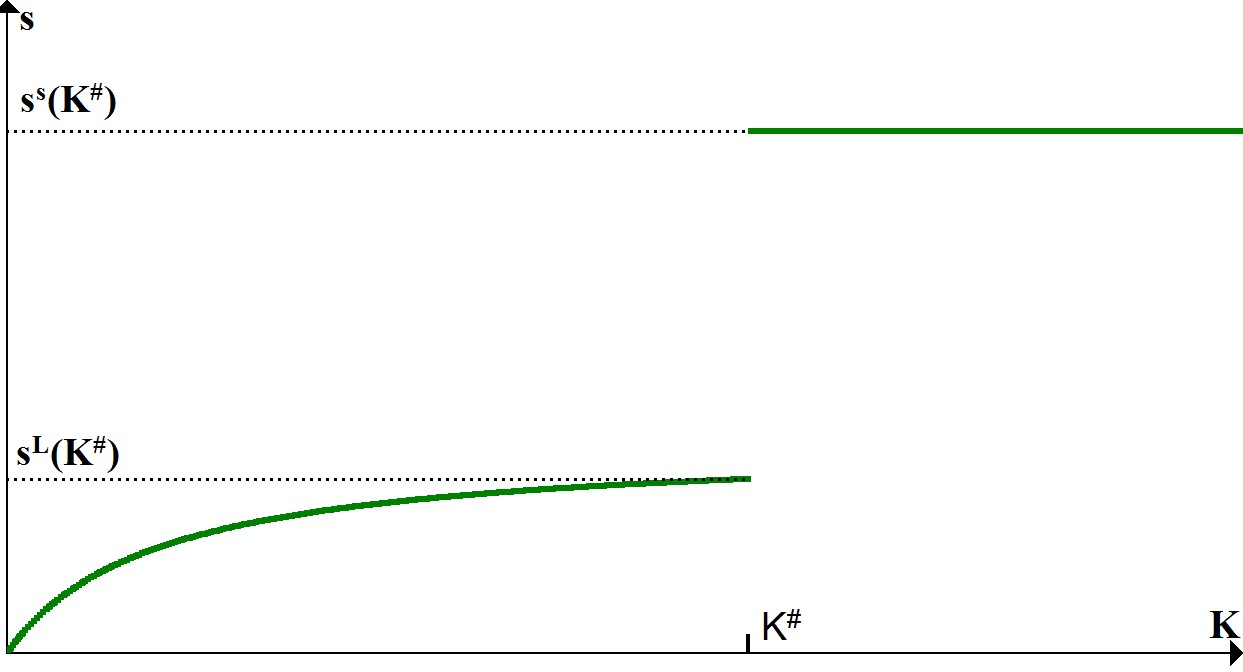
\includegraphics[width=\textwidth]{EndoSavings.jpg}
\caption{saving rate as a function of $K$.}
\end{figure}
\newline
\noindent The saving rate is a smooth function over the Lewis range, i.e. $K<K^{\#}$, (it rises because the mature sector becomes an increasingly large part of the economy), but is discontinuous at the point where the Solow range is entered. There is no economic reason for this sudden hike and hence it is a problem we need to resolve if we want to link both models. Several possibilities are available.

\subsection{Adjust the Solow Model}

In the Solow model, one could define savings on the basis of profits instead of total income: set $s_{\pi}^S=s_{\pi}^L$. We know that the total income of capitalists equals a fraction ${\alpha}$ of total income (as a result of the Cobb-Douglas production function). Hence, this adjustment comes down to setting $s^S={\alpha}s_{\pi}^s$, a factor ${\alpha}$ lower than before. The gap in the savings function at $K^{\#}$ in figure 1 will disappears (see figure 2).
\begin{figure}[!ht]
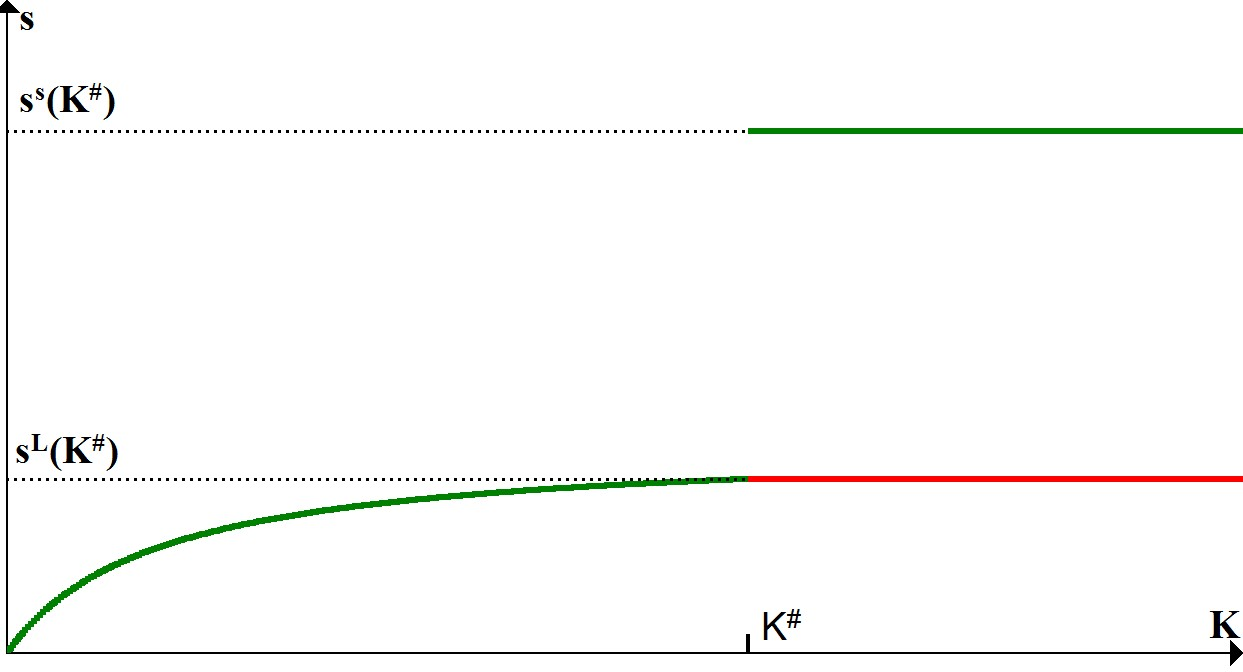
\includegraphics[width=\textwidth]{EndoSavings1.jpg}
\caption{In the Solow range $s$ shifts downward to the red line.}
\end{figure}\\
Obviously, the dynamics over the Lewis range remain unaltered, since no variable has changed in that dimension. With respect to the Solow range, the smaller saving fraction means that the rate of capital accumulation decreases...

\begin{align}
\hat{k}={\alpha}s^{S}k^{\alpha-1}-\delta<s^{S}k^{\alpha-1}-\delta
\end{align}
...as well as lowering the steady-state income level:
\begin{align}
y^*=({\alpha}s^{S}/\delta)^{\alpha/({1-\alpha})}<(s^{S}/\delta)^{\alpha/({1-\alpha})}
\end{align}
\subsection{Adjust the Lewis Model I}
The reversed case is to use mature sector income $Y_m$ as the basis for savings in the Lewis model, i.e. $s_{Y_m}=s^S$ , mirroring the total income savings rate of the Solow model. Again, given the Cobb-Douglas production function, profits equal a fraction ${\alpha}$ of mature income. Thus, this modification is similar to selecting $s_{\pi}^L=s_{Y_m}/{\alpha}$, inflating $s_{\pi}^L$ by a factor $1/{\alpha}$ compared to before. Graphically, the part of the savings curve before maturity is shifted upwards and the discontinuity has disappeared (see figure 3).\\
From equation (15b) it is clearly visible that the rate of capital growth increases by taking a broader basis for our savings. As a consequence, total income $Y_m+Y_s$ grows faster as well, see equation (19b). This change in dynamics over the Lewis range is displayed in figure 4.
\begin{figure}[!ht]
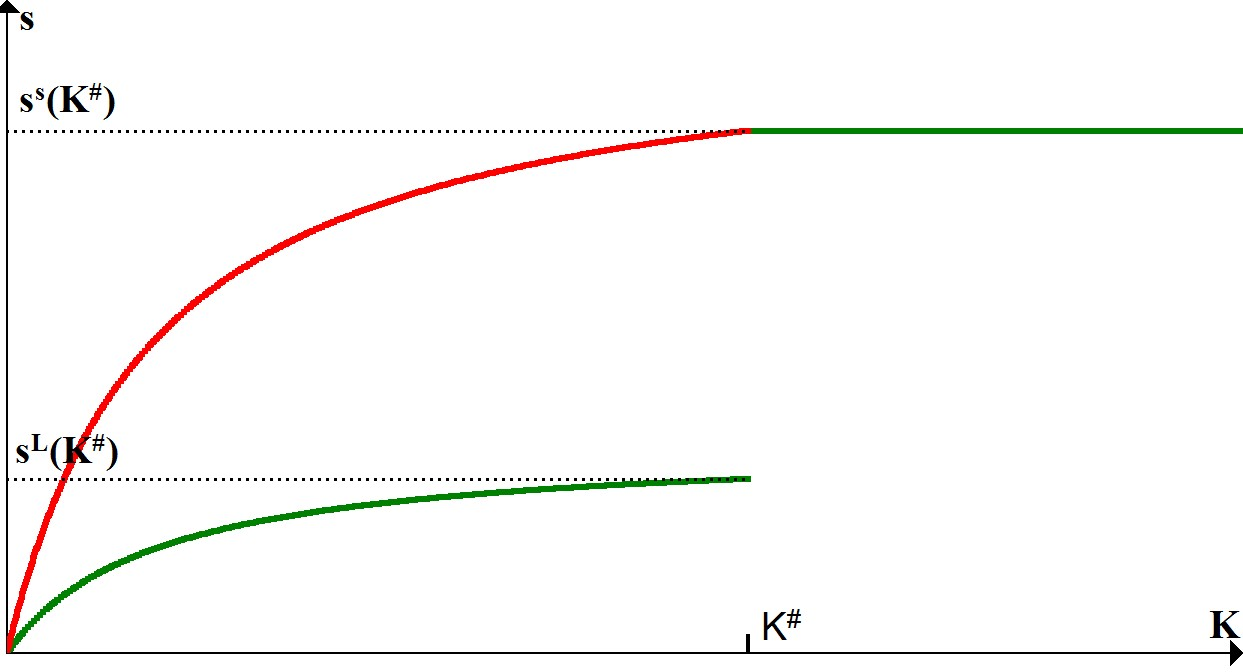
\includegraphics[width=\textwidth]{EndoSavings2.jpg}
\caption{In the Lewis range $s$ shifts upward to the red line.}
\end{figure}\\
\begin{figure}[!ht]
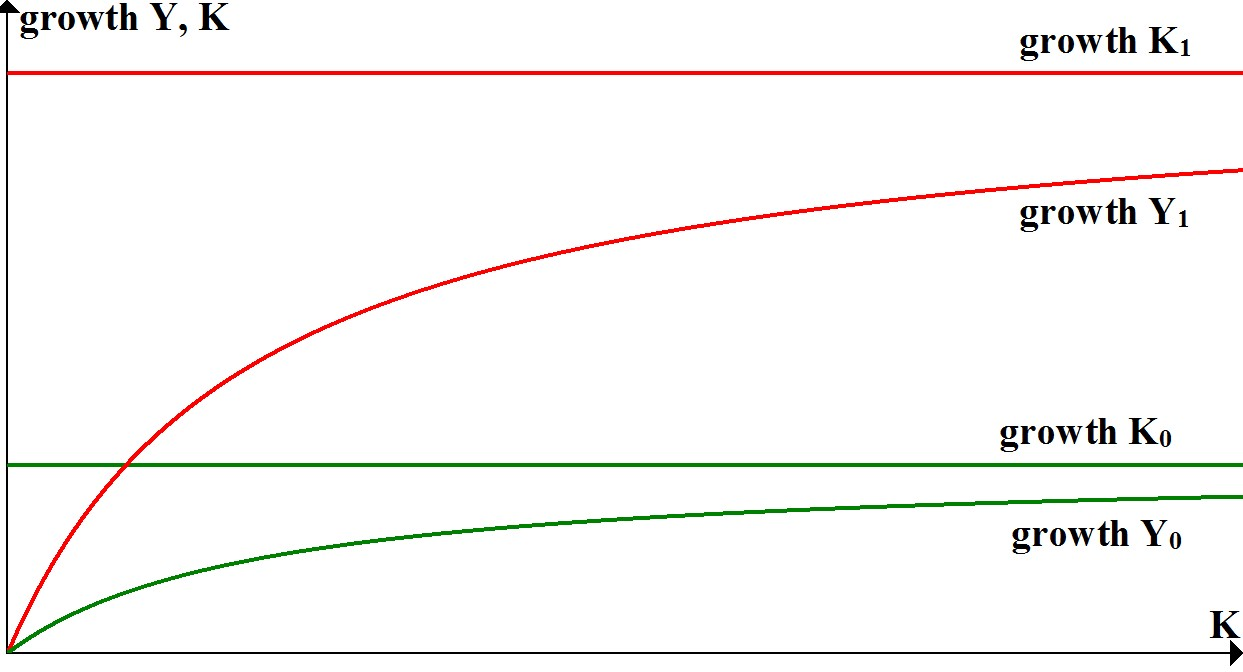
\includegraphics[width=\textwidth]{Growth1.jpg}
\caption{Comparison of growth rates of Y and K over the Lewis range: savings rate based on profits (green) versus  savings rate based on mature income (red).}
\end{figure}
\newpage
\subsection{Adjust the Lewis Model II}

Instead of focusing solely on income in the mature sector, one could involve the subsistence sector as well: use $Y_m+Y_s$ as the basis for the saving rate in the Lewis model. This amounts to setting $s^L=s^S$. As a percentage of total income, the savings rate in the Lewis range is now no longer increasing with $K$, instead it will be a constant function. Naturally this eliminates any discontinuity issues (see also figure 5).
This adjustment has much larger consequences compared to the previous two cases: we have to reformulate the complete dynamics of the model, instead of simply changing one parameter. The capital accumulation equation now becomes:
\begin{subequations}
\begin{alignat}{2}
 &\dot{K} 	&&\hspace{-0.1cm}=s^LY-{\delta}K\nonumber\\
 &{}		&&\hspace{-0.1cm}=s^LA_sL+s^LKA_s({\phi}/(1-{\alpha})-1)((1-{\alpha})A_m/{\phi}A_s)^{1/{\alpha}}-{\delta}K\\
 \Rightarrow \hspace{0.1cm} 
 &\hat{K}	&&\hspace{-0.1cm}=s^LA_sL/K+s^LA_s({\phi}/(1-{\alpha})-1)((1-{\alpha})A_m/{\phi}A_s)^{1/{\alpha}}-{\delta}
\end{alignat}
\end{subequations}
Hence capital does no longer grow at a constant rate.\\
\begin{figure}[!ht]
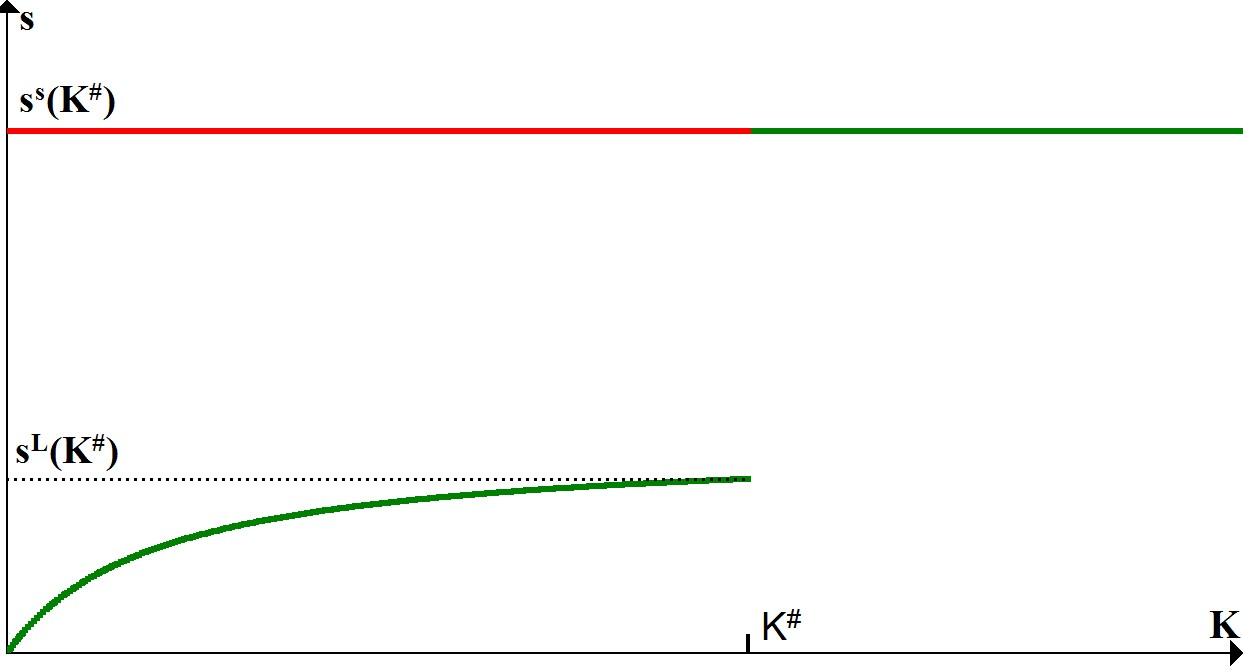
\includegraphics[width=\textwidth]{EndoSavings3.jpg}
\caption{In the Lewis range $s$ shifts upward to the red line.}
\end{figure}\\

\newpage
\section{Unified Growth: from Lewis to Solow}
\textit{Show the dynamics of an economy that starts with small capital stock and surplus labour and show how it can finally reach the "mature stage"where the economy behaves like the Solow model. Show how the dynamics of the two regimes are linked. Derive equations for (and plot) profits, output, wages, etc. as  a function of the captial stock, ditinguishing between the Lewis range $(K<K^{\#})$ and the Solow range $(K>K^{\#})$. Generate time patterns etc. Make sure that the assumption about savings allows you to really connect the two models: e.g. assume that always a fixed fraction of profits is reinvested (even in the Solow regime), or assume that up to a threshold per captia income level is saved, but a fixed fraction of the remaineder of income.}\\
\newline
Given our discussion of the saving rate issue in part 2, we will have to select one of the discussed adjustments to provide the required numerical example of the Lewis-Solow-dynamics. The third option, setting $s^L=s^s$, seems somewhat less logical: the very idea behind the subsistence sector is that income is at ‘subsistence level’, which leaves no scope for saving. The two remaining options are very much alike, so we simply opt for the first option, imposing $s_\pi^s=s_\pi^L$.\\
\newline
\noindent\textbf{The assignment includes several more pages, however, no new commands are required for the remainder from here on. I hope the above proves my proficiency with Latex sufficiently.}
\end{document}
